%------------------------------------------------------------------------
%Editar Diplomado
\hypertarget{cv:modificarCU}{\section{Modificar Caso de Uso}} \label{sec:modificarCU}

	Esta funcionalidad le permitirá modificar la información de un caso de uso previamente registrada con el fin de corregir o actualizar datos del mismo. 

		\subsection{Procedimiento}

			%Pasos de procedimiento
			\begin{enumerate}
	
			\item Oprima el botón \IUEditar{} de algún registro existente de la pantalla \ref{fig:GestionarCU} ''Gestionar Casos de Uso''.
	
			\item Se mostrará la pantalla \ref{fig:modificarCUA} ''Modificar Caso de Uso''.
			
			%Pantalla
			\begin{figure}[H]
				\begin{center}
					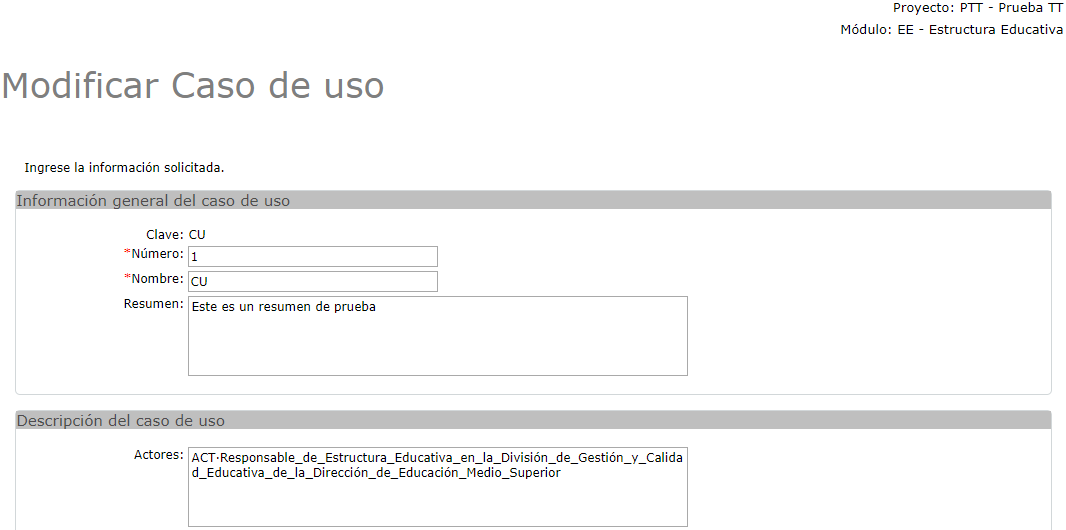
\includegraphics[scale=0.5]{roles/lider/casosUso/pantallas/IU12-2modificarCUA}
					\caption{Modificar Caso de Uso}
					\label{fig:modificarCUA}
				\end{center}
			\end{figure}
		
			%Pantalla
			\begin{figure}[H]
				\begin{center}
					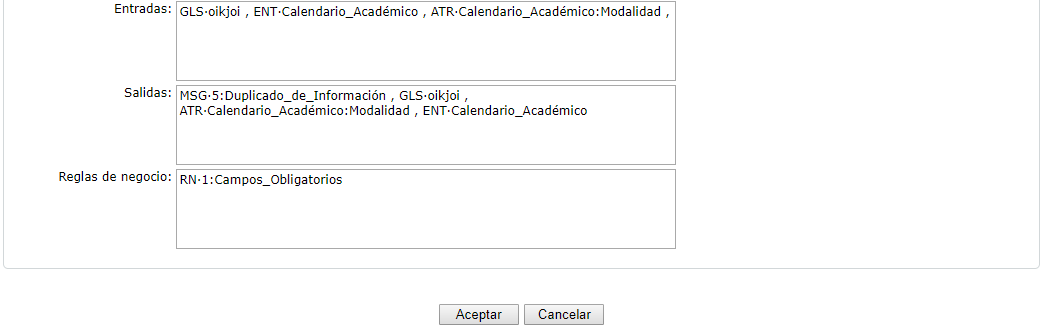
\includegraphics[scale=0.6]{roles/lider/casosUso/pantallas/IU12-2modificarCUB}
					\caption{Modificar Caso de Uso}
					\label{fig:modificarCUB}
				\end{center}
			\end{figure}
		
			\item Modifique los datos solicitados por la pantalla.
			
			\item Para la sección de ''Descripción del caso de uso'' podrá ingresar TOKENS para vincular diferentes elementos previamente registrados dependiendo de cada campo en el que se encuentre:
			
			\begin{itemize}
				\item En el campo de actores solo podrá referenciar elementos de tipo actor con el TOKEN: ''ACT·''.
				\item En el campo de entradas solo podrá referenciar elementos de tipo entidad, atributos y términos de glosario con los TOKEN: ''ENT·'', ''ATR·'' y ''GLS·''.
				\item En el campo de salidas solo podrá referenciar elementos de tipo entidad, atributos y términos de glosario con los TOKEN: ''ENT·'', ''ATR·'', ''GLS·'' y ''MSG·''.
				\item En el campo de reglas de negocio solo podrá referenciar elementos de tipo regla de negocio con el TOKEN: ''RN·''.
			\end{itemize}
						
			\item Oprima el botón \IUAceptar.
			
			\item Se mostrará el mensaje \ref{fig:CUModificado} en la pantalla \ref{fig:GestionarCU} ''Gestionar Casos de Uso''.
			
			\begin{figure}[htbp!]
				\begin{center}
					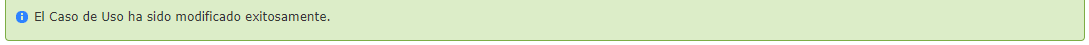
\includegraphics[scale=0.56]{roles/lider/casosUso/pantallas/IU12-2MSG1}
					\caption{MSG: Caso de Uso Actualizado}
					\label{fig:CUModificado}
				\end{center}
			\end{figure}
			\end{enumerate}